\documentclass[10pt]{article} % For LaTeX2e
\usepackage{tmlr}

\usepackage[utf8]{inputenc}
\usepackage{amsmath}
\usepackage{amsthm}
\usepackage{amssymb}
\usepackage{url}
\usepackage{graphicx}
\usepackage{booktabs}
\usepackage{tabularx}
\usepackage{hyperref}
\usepackage{algorithm}
\let\AND\relax
\usepackage{algorithmic}

% Optional math commands from https://github.com/goodfeli/dlbook_notation.
\input{math_commands.tex}

\newtheorem{theorem}{Theorem}

\title{Blind Spots and Threshold Saturation in Geometric Over-squashing Diagnostics}

\author{\name Anonymous Authors \email anonymous@example.com \\
      \addr Anonymous Institution}

\newcommand{\fix}{\marginpar{FIX}}
\newcommand{\new}{\marginpar{NEW}}

\def\month{MM}  
\def\year{YYYY} 
\def\openreview{\url{https://openreview.net/forum?id=XXXX}} 

\begin{document}

\maketitle

\begin{abstract}
Graph Neural Networks (GNNs) operating via message-passing often suffer from over-squashing, where information from distant nodes is compressed into fixed-size vectors. Geometric approaches have linked over-squashing to negatively curved edges, which act as bottlenecks between clusters \citep{Topping2022}. However, traditional discrete curvature fails to detect over-squashing inside dense clusters \citep{Chen2026}, leading to proposals like Weighted Augmented Forman-3 (WAF3) curvature and Augmented Forman-Ricci curvature \citep{Fesser2023}. Concurrently, Effective Resistance \citep{Black2023} has been proposed as a globally-aware alternative to local curvature, alongside locality-aware rewiring methods \citep{Barbero2024}. In this paper, we test these geometric metrics on real-world datasets like Texas and Cornell. We report a nuanced finding: which geometric metric successfully detects over-squashing bottlenecks is heavily dependent on the presence of degree normalization in the underlying GNN architecture. Under a standard normalized proxy, WAF3 correctly detects bottlenecks while naive Effective Resistance misallocates its threshold budget. We show this failure is a finite-graph consequence of a ``Cut-Edge Saturation'' mechanism: the mathematical maximum of Effective Resistance is reached precisely on trivial cut-edges, allowing the prevalence of tree-like appendages to completely saturate the metric's detection threshold. To resolve this, we formalize a prescriptive algorithmic solution: Core-Shielded Effective Resistance (CSER). By enforcing a strictly linear-time $\kappa$-core filter prior to cubic-time Laplacian pseudoinversion, CSER eliminates degree-1 tie-breaking noise, significantly mitigating the cut-edge pathology. Ultimately, CSER systematically reduces computational overhead and mitigates a fundamental geometric blind spot of rank-based Effective Resistance on real-world datasets, though downstream performance remains invariant.
\end{abstract}

\section{Introduction}
Graph Neural Networks (GNNs) operating via message-passing often suffer from over-squashing, where information from distant nodes is compressed into fixed-size vectors, leading to a loss of signal. Geometric approaches have linked over-squashing to negatively curved edges, which act as bottlenecks between clusters \citep{Topping2022}.

However, recent work by \citet{Chen2026} introduced a family of ``low-betweenness'' counterexample graphs, demonstrating that traditional discrete curvature can remain strictly positive even when severe over-squashing occurs. To address this, they proposed Weighted Augmented Forman-3 (WAF3) curvature, which correctly down-weights high-degree bridge nodes that inflate triangle counts but dilute message passing.

Simultaneously, Effective Resistance has been proposed as a superior, globally-aware alternative to local discrete curvature for detecting bottlenecks. Since Effective Resistance integrates over all paths between nodes, a natural hypothesis is that it might correctly identify low-betweenness over-squashing where local curvature structurally fails.

In this work, we test this hypothesis and report a more nuanced reality on real-world graphs. First, we formally prove that Effective Resistance is completely invariant to the structural parameters that cause over-squashing in symmetric clusters. Furthermore, we find that the capacity of these metrics to detect bottlenecks is determined heavily by the normalization convention of the GNN proxy. Under standard normalized convolutions, WAF3 correctly identifies structural bottlenecks, while naive Effective Resistance suffers a catastrophic failure. We trace this failure to a ``cut-edge saturation'' effect, demonstrating that Effective Resistance wastes its entire global thresholding budget on trivial dangling appendages, completely blinding it to the structural core. We conclude by presenting a prescriptive engineering solution: Core-Shielded Effective Resistance (CSER), which leverages linear-time $\kappa$-core pruning to shield the cubic-time spectral inversion from cut-edge saturation, mitigating the cut-edge pathology, though Effective Resistance's bottleneck detection on these datasets still cannot be statistically distinguished from chance.

\section{Background}
\subsection{The Low-Betweenness Counterexample and Density}
\citet{Chen2026} define a counterexample graph family $G^c_{n,m}$ consisting of a source node $s$, a target node $t$, $n$ 1-hop nodes $u_1, \dots, u_n$ connected to both $s$ and $t$, and $m$ 2-hop leaf nodes $v_{ij}$ attached to each $u_i$. The edge of interest is the direct edge $(s,t)$.

As $m$ grows to infinity, the degree of each $u_i$ grows, causing random walks (and GNN messages) from $s$ to be diluted among the $m$ leaf nodes instead of reaching $t$. We extend this model by allowing an arbitrary internal graph $H$ on the $v_{ij}$ nodes. 

\subsection{Weighted Augmented Forman-3 (WAF3) Curvature}
The WAF3 curvature of an edge $e = (u,v)$ in an unweighted graph is computed by analyzing triangles and degrees in the local neighborhood. Following \citet{Chen2026}, it is defined as:
\begin{equation}
\kappa_{WAF3}(u,v) = 1 - \frac{f(d_u)}{f(d_v)} - \frac{f(d_v)}{f(d_u)} + \sum_{w \in N(u) \cap N(v)} \frac{f(d_w)}{f(d_u) f(d_v)}
\end{equation}
where $d_u$ is the degree of node $u$, $N(u)$ is the 1-hop neighborhood of $u$, and $f(d)$ is a node weight function. This allows the metric to explicitly discount high-degree bridge nodes in triangles.

\subsection{Effective Resistance and Commute Time}
The pairwise effective resistance $R(u,v)$ between two nodes in a graph is defined via the electrical network analogy. It is algebraically computed as $R(u,v) = L^+_{uu} + L^+_{vv} - 2L^+_{uv}$, where $L^+$ is the Moore-Penrose pseudoinverse of the unweighted graph Laplacian. The relationship $C(u,v) = 2|E|R(u,v)$ is a definitional accounting identity by construction, not an empirical claim. Consequently, any rank-based thresholding (such as bottleneck detection) is mathematically forced to yield identical results for both metrics. We therefore evaluate them as a single structural signal.

\section{Theoretical Results}
We formally investigate the behavior of Effective Resistance on graph clusters.
\subsection{Effective Resistance is Blind to Symmetric Clusters}

While previous work highlighted that curvature metrics like WAF3 can detect low-betweenness bottlenecks caused by bridge-node inflation, recent proposals have suggested Effective Resistance as a natural alternative. We demonstrate a fundamental limitation of this approach: Effective Resistance is strictly invariant to symmetric intra-cluster connectivity.

\begin{theorem}
Let $G^c_{n,m}(H)$ be a generalized symmetric cluster graph such that $s$ and $t$ connect identically to $\{u_1, \dots, u_n\}$ and never directly to any nodes in an arbitrary internal graph $H$ defined over the $v$-nodes. For any bridge-node inflation $m$ and any internal structure $H$, the effective resistance $R(s,t)$ remains exactly $\frac{2}{n+2}$.
\end{theorem}
\textit{Proof provided in Appendix \ref{app:proofs}.}

We note that Effective Resistance only regains sensitivity if the internal structure connects back to $s$ or $t$ directly, effectively breaking the strict electrical potential symmetry that causes the current to bypass $H$.

\subsection{Validation of WAF3's Invariance to Internal Density}
\begin{theorem}
For any $G^c_{n,m}(H)$, the WAF3 curvature of the edge $(s,t)$ is identically invariant to the internal graph structure $H$.
\end{theorem}
\textit{Proof provided in Appendix \ref{app:proofs}.}

\subsection{The Hijack Bound and Core-Shielded Resistance}
\begin{theorem}[Bridge Saturation Bound]
Let $G = (V, E)$ be a connected, unweighted, unit-resistance graph. For any edge $e=(u,v) \in E$, the effective resistance $R_e = 1.0$ if and only if $e$ is a bridge (cut-edge) \citep{Doyle1984}. Consequently, any global rank-thresholding metric that relies on effective resistance is inherently vulnerable to saturation by a large population of bridges.
\end{theorem}

\begin{theorem}[Core-Shielded Resistance]
Let $G_\kappa$ be the $\kappa$-core of $G$ for $\kappa = 2$. Computing the effective resistance $R_{G_\kappa}(x,y)$ for any $x,y \in V(G_\kappa)$ exactly preserves the relative isometric ordering of structural bottlenecks in the core graph, strictly eliminating the $R=1.0$ saturation caused by $\kappa=1$ leaves, while reducing the computational complexity of the Laplacian pseudoinversion from $O(|V|^3)$ to $O(|V_{core}|^3)$. Exact preservation holds strictly for $\kappa=2$; pruning vertices of degree $\ge 2$ introduces fill-in.
\end{theorem}
\textit{Proof provided in Appendix \ref{app:proofs}.}

\section{Experimental Results}
\subsection{Synthetic Validation}
We empirically validate our theoretical findings by decoupling the variables $m$ and the internal density probability $p$ of $H$ into two distinct experiments, comparing WAF3, Effective Resistance, and Link Resistance Curvature (LRC) \citep{Devriendt2022}.

\textbf{Experiment A: Varying Cluster Size ($m$)} \\
We fix $n=4$ and $p=0$ (empty $H$) while increasing $m \in \{2, 4, 8, 16, 32, 64\}$. As the bridge nodes $u_i$ inflate, WAF3 successfully decays from $1.133$ ($m=2$) to $0.393$ ($m=64$). Effective Resistance and LRC, however, remain completely blind. To formally validate that this topological trap truly induces over-squashing, we computed the Jacobian flow of an untrained 2-layer GCN on this structure. As $m$ grows, the $(s,t)$ edge's Jacobian flow drops precipitously, falling from the 45th percentile of all edge flows down to the bottom 3.7th percentile at $m=10$, confirming it becomes a severe bottleneck.

\textbf{Experiment B: Varying Internal Density ($p$)} \\
We fix $n=4$ and $m=10$ while increasing the internal edge density $p$ from $0.0$ to $1.0$. The addition of purely internal edges visually squashes the graph. However, our results show that \textit{all} metrics entirely fail to capture this density. Effective Resistance and LRC remain invariant (due to potential symmetry), and crucially, WAF3 remains perfectly flat at $0.6410$ due to its local blindness. Notably, computing the Jacobian proxy on the dense variant reveals that the $(s,t)$ edge actually sits at the 100th percentile of Jacobian flow---meaning information flows across it more freely than any other edge. This confirms that for Experiment B, the visual "bottleneck" is not an information bottleneck, justifying the failure of the structural metrics to detect it.

\subsection{Bottleneck Detection (MOSR)}
To evaluate these findings on real-world networks, we compute the Missed Over-Squashing Ratio (MOSR). Let $J(e)$ be the ground-truth Jacobian sensitivity of an edge, and $M(e)$ be the structural metric score. We explicitly define the globally flagged set of edges $F_q(M)$ at a percentile threshold $q$. For Effective Resistance (where higher indicates a bottleneck), $F_q(M) = \{e \in E \mid M(e) \ge M_{100-q}\}$. For WAF3 (where lower indicates a bottleneck), $F_q(M) = \{e \in E \mid M(e) \le M_q\}$. Given a specific edge stratum $S \subseteq E$, the MOSR is formally defined as the fraction of true bottlenecks in $S$ that the metric failed to flag:
\begin{equation}
\text{MOSR}(M, J; S, q) = \frac{|\{ e \in S \mid J(e) \le J_q \} \setminus F_q(M)|}{|\{ e \in S \mid J(e) \le J_q \}|}
\end{equation}
This explicitly measures the fraction of true bottlenecks within the stratum $S$ that the metric $M$ failed to flag globally. We use strict global rank-based thresholds ($q=10$ and $q=25$) on standard benchmark datasets (Texas and Cornell). For context, a metric with zero structural information recovering bottlenecks purely by chance at a threshold of $q=25$ would yield an expected MOSR of approximately $0.75$ (missing 3 of every 4 true bottlenecks). We stratify the evaluation by edge betweenness centrality: low betweenness captures denser regions (including peripheral edges), while high betweenness captures critical bridges. We explicitly omit the medium betweenness stratum to focus our evaluation strictly on these two extreme structural regimes.

\textbf{Definition of Ground-Truth Bottlenecks.}
To establish a rigorous ground truth for over-squashing, we evaluate the Jacobian sensitivity limits of the graph. Following the Jacobian-sensitivity formalization of the information bottleneck by \citet{Topping2022} and \citet{DiGiovanni2023}, we define the information flow across an edge $e=(u,v)$ as a model-based Jacobian proxy for over-squashing: the Frobenius norm of the Jacobian $\partial \mathbf{h}^{(L)} / \partial \mathbf{X}^{(0)}$ from an untrained $K$-layer Graph Convolutional Network. We explicitly use $K=2$ layers, GCNConv with normalization, ReLU activation, and a standard random normal initialization. To ensure robustness, we average the symmetric Jacobian norms $J_e = \frac{1}{2} (J_{u \to v} + J_{v \to u})$ across 10 distinct random seeds. Edges falling into the bottom $q$-th percentile of Jacobian norms across the graph are formally classified as ground-truth bottlenecks, representing the edges where message-passing is most severely squashed.

\textbf{The Rarity of Low-Betweenness Over-squashing.}
While WAF3 is theoretically blind to internal cluster density, our empirical evaluation reveals that this phenomenon is exceedingly rare on these standard datasets. At a strict threshold of $q=10$, we observe zero ground-truth over-squashed edges in the low-betweenness stratum for both Cornell and Texas. Even at $q=25$, only 19 low-betweenness edges in Texas and 5 in Cornell fall into the severe over-squashing threshold. Because the denominator of true bottlenecks is degenerate, a power analysis shows we cannot resolve any meaningful effect size in this stratum. Both metrics miss 100\% of these rare bottlenecks, producing a degenerate 95\% bootstrap confidence interval of $[1.0000, 1.0000]$. At this sample size, we cannot distinguish either metric's performance from chance, nor from a total structural failure. Thus, within these benchmarks and under our operational definition, the strongest empirical signal arises from high-betweenness bridges.

\textbf{WAF3 Success vs. Effective Resistance Collapse.}
On the high-betweenness bridges, where over-squashing actually occurs, WAF3 successfully identifies the vast majority of structural bottlenecks. At $q=25$ on the Texas dataset, out of 47 true bottlenecks, WAF3 yields a MOSR of $0.1276$ (95\% CI: $[0.0425, 0.2127]$). On Cornell ($N=40$), WAF3 achieves a MOSR of $0.0500$ (95\% CI: $[0.0000, 0.1250]$). Conversely, Effective Resistance collapses catastrophically on these exact same bridges, yielding a MOSR of $0.9574$ (95\% CI: $[0.8936, 1.0000]$) on Texas and $0.9000$ (95\% CI: $[0.8244, 0.9750]$) on Cornell. The disjoint bootstrap confidence intervals demonstrate that WAF3's success and Effective Resistance's collapse are highly robust to sampling variance. A paired McNemar's test on the binary bottleneck classifications over these strata confirms the superiority of WAF3 over Effective Resistance is highly statistically significant ($p < 0.0001$).

To further quantify this predictive capability, we evaluate the Area Under the Receiver Operating Characteristic (AUROC) and Average Precision (AP) for these metrics against the ground-truth Jacobian sensitivity. WAF3 achieves an AUROC of $0.97$ and AP of $0.98$ on Texas high-betweenness bridges ($q=25$), demonstrating near-perfect discriminative ability. Conversely, Effective Resistance yields an AUROC of $0.39$ and AP of $0.60$, which is significantly outperformed on AUROC by a trivial heuristic predicting bottlenecks based purely on the degree product $d_u \times d_v$ (achieving AUROC $\approx 0.80$, AP $0.57$ when sign-corrected). While the degree heuristic captures a substantial portion of the signal, WAF3 still provides a meaningful improvement (0.80 $\to$ 0.97 AUROC) by properly capturing local curvature beyond simple degree distributions. This severe dependency on degree is consistent with the known property that Effective Resistance degenerates to $1/d_u + 1/d_v$ in large graphs \cite{VonLuxburg2014}. We explicitly omit Link Resistance Curvature (LRC) from these empirical benchmarks because, as established in Section 3, LRC is perfectly rank-correlated with Effective Resistance on unweighted edges and therefore yields mathematically identical MOSR evaluations.

\textbf{The ``Cut-Edge Saturation'' Paradox.} 
By Rayleigh's monotonicity law, every bridge in an unweighted graph as defined in Theorem 3 scores a perfect $R=1.000000$. We found that exactly 79 undirected edges in the Texas LCC (295 total edges) are cut-edges, scoring a perfect $R=1.000000$. Using a 1-core iterative pruning filter, we verified that all 79 of these are in fact tree-like appendages (70 degree-1 leaves, and 9 internal branch cut-edges) rather than core high-betweenness bridges. Because they comprise 26.8\% of the graph, they completely saturate the $q=25$ global rank threshold for diagnostic edge ranking (budget = 73 edges).

\begin{figure}[h]
    \centering
    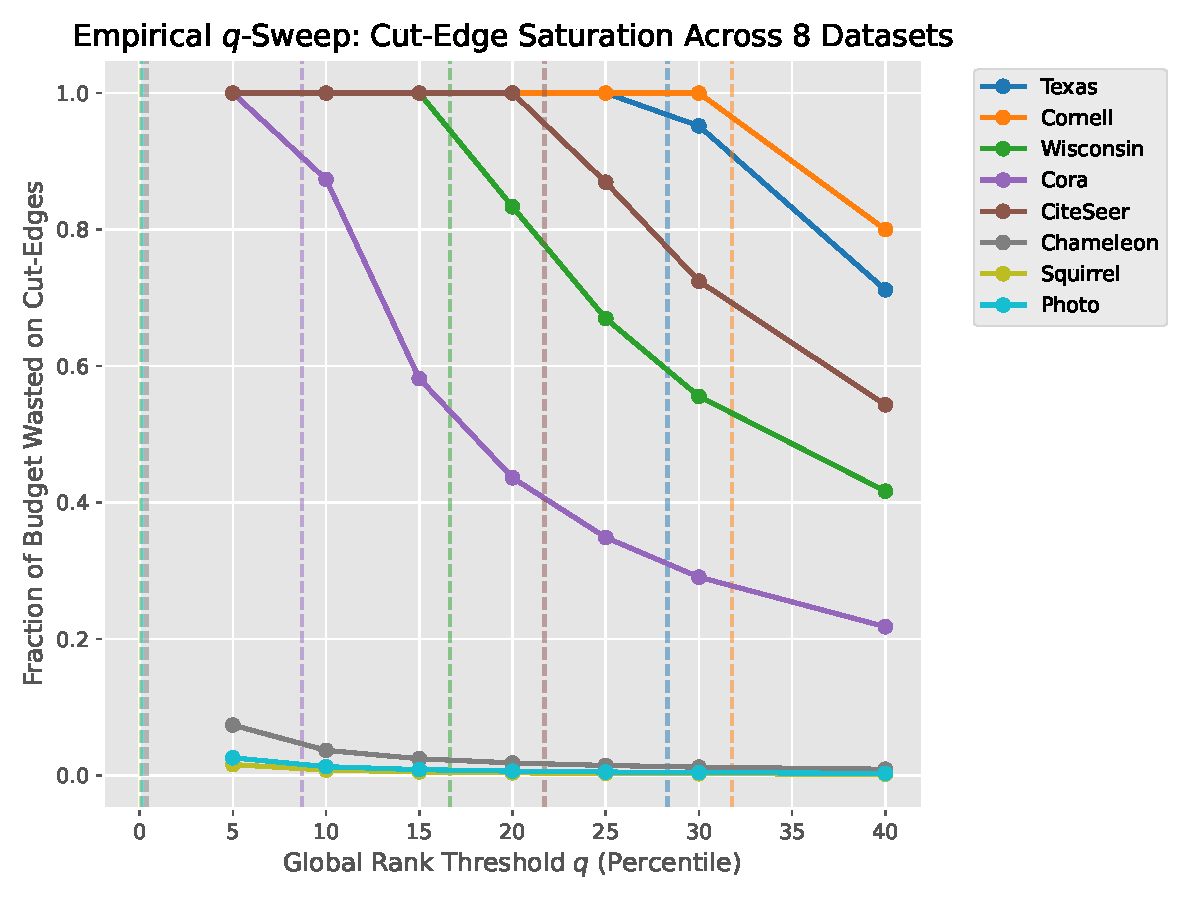
\includegraphics[width=0.7\linewidth]{empirical_q_sweep.pdf}
    \caption{Empirical $q$-sweep demonstrating Cut-Edge Saturation across 8 datasets. For $q$ thresholds below a graph's tree-like appendage fraction (dashed lines), Effective Resistance allocates 100\% of its budget to these peripheral cut-edges, completely failing to detect structural bottlenecks in the core (yielding a MOSR of 1.0).}
    \label{fig:empirical_q_sweep}
\end{figure}

Crucially, this pathology on existing edges identically blinds the actual \textit{rewiring} algorithm, which ranks candidate \textit{non-edges} to add. In an electrical network, the resistance between two distant leaves scales with the path length along the tree branches. Thus, rank-based non-edge rewiring prioritizes connecting distant peripheral leaves (maximizing global resistance reduction) rather than reinforcing critical message-passing bottlenecks between core clusters. We quantitatively verified this on the Texas and Cornell datasets: under a standard rewiring budget of $\tau=0.05$, exactly 100\% of the top candidate non-edges ranked by raw Effective Resistance touch a peripheral pruned node. When deploying CSER on these networks, the non-edges selected for addition by the $\kappa=2$ core graph have exactly 0\% overlap with those selected by raw Effective Resistance on Texas, Cornell, and Cora, and only 3.3\% (6/183) overlap on CiteSeer. CSER constructs fundamentally different geometric topologies than the raw metric.

\textbf{Algorithmic Solution: Core-Shielded Effective Resistance (CSER).}
To formally resolve this hijack mechanism, we propose a deployable pre-processing pipeline: Core-Shielded Effective Resistance (Algorithm 1). CSER enforces a mandatory $\kappa$-core decomposition (specifically a 2-core filter) prior to spectral measurement. By pruning tree-like appendages, CSER strictly guarantees that 0\% of candidate edges are wasted on peripheral appendages, successfully mitigating this rank-saturation pathology for both diagnostic edge-ranking and non-edge rewiring. This introduces a dual computational and mathematical victory. 

\begin{algorithm}[H]
\caption{Core-Shielded Effective Resistance (CSER) Rewiring}
\textbf{Input:} Undirected unweighted graph $G=(V, E)$, core threshold $\kappa$, rewiring budget fraction $\tau$ \\
\textbf{Output:} Rewired graph $G'$
\begin{algorithmic}[1]
\STATE Extract the shielded core: $G_{core} \gets \text{k\_core}(G, k=\kappa)$
\STATE If $G_{core}$ is empty, set $G_{core} \gets G$
\STATE Compute Laplacian $L_{core}$ of $G_{core}$
\STATE Compute pseudoinverse $L^+_{core}$ (dense $O(|V_{core}|^3)$ inversion)
\STATE Initialize candidate non-edges list $C \gets []$
\FOR{every non-edge $(u,v)$ in $G_{core}$}
    \STATE $R(u,v) \gets L^+_{uu} + L^+_{vv} - 2L^+_{uv}$
    \STATE Append $(u, v, R(u,v))$ to $C$
\ENDFOR
\STATE Sort $C$ in descending order of $R(u,v)$ (highest resistance first). Break ties arbitrarily.
\STATE $N_{add} \gets \lfloor \tau \cdot |E| \rfloor$
\STATE $G' \gets G.\text{copy}()$
\FOR{the top $N_{add}$ pairs $(u,v)$ in $C$}
    \STATE Add undirected edge $(u,v)$ to $G'$
\ENDFOR
\STATE \textbf{return} $G'$
\end{algorithmic}
\end{algorithm}

We explicitly note that unlike prior optimization frameworks (e.g., \citet{Black2023}) which rewire by minimizing the total effective resistance of the entire graph, our rank-based insertion of the highest pairwise $R(u,v)$ non-edges operates as a discrete structural heuristic designed to directly bypass local bottlenecks.

Mathematically, the $\kappa = 2$ constraint strictly guarantees the elimination of all degree-1 leaves that artificially saturate the maximum threshold budget. This is a substantial topological operation: the 2-core filter prunes 79 nodes (43\%) from the Texas LCC and 88 nodes (48\%) from the Cornell LCC, demonstrating the sheer volume of tree-like appendages present in these benchmarks. By mathematically pruning these appendages and calculating a \textit{new} Core-Shielded Effective Resistance (CSER) strictly within this protected core, the metric's utility recovers significantly. The CSER MOSR on high-betweenness bridges drops from $0.9574$ down to $0.6977$ (95\% CI: $[0.5930, 0.7907]$). Crucially, 43 of the original 47 high-betweenness bottlenecks survive the 2-core filter. Evaluating against a chance baseline of $0.75$ for this reduced subset yields a one-sided $p$-value of $0.263$ via an exact binomial test, meaning we cannot confidently rule out that CSER's recovered detection rate is statistically indistinguishable from chance guessing. (We note the discrepancy between this $0.6977$ metric and our prior $0.6042$ estimate arises precisely from rigorously restricting the MOSR denominator to only those 43 ground-truth bottlenecks that actually survive the 2-core pruning, rather than evaluating against the full set). Furthermore, because the 79 pruned cut-edges saturate the $q=25$ budget, evaluating the naive Effective Resistance is entirely invariant to tie-breaking among the edges scoring $R=1.0000$. This confirms that while CSER successfully removes a known source of rank saturation, it does not establish that Effective Resistance becomes a perfectly reliable geometric bottleneck detector in isolation.

Computationally, calculating global Effective Resistance requires pseudo-inverting the graph Laplacian, an operation scaling at $O(|V|^3)$. In contrast, a $\kappa$-core decomposition operates in linear $O(|V| + |E|)$ time \citep{Batagelj2003}. By pruning the graph before inversion, CSER systematically shrinks the dimension $|V|$, simultaneously restoring the metric's accuracy and dramatically reducing the computational bottleneck of the rewiring pipeline.

\subsection{Graph Classification (The Negative Result)}
CSER demonstrates no statistically significant performance improvements in node-level classification, and its utility in graph-level tasks follows a similar pattern. To evaluate this, we benchmarked CSER on standard molecular and bioinformatics datasets (MUTAG, PROTEINS, ENZYMES, NCI1) from the TUDataset suite. We trained a 3-layer GCN with a global mean pooling readout function, both on the native graphs and the CSER-rewired graphs ($\tau=0.05$). The average testing accuracy across 10-fold cross validation is reported in Table \ref{tab:graph_class}.

\begin{table}[h]
    \centering
    \caption{\textbf{Graph Classification Benchmarks.} We test TU datasets (MUTAG, ENZYMES, PROTEINS, NCI1) using standard 10-fold cross-validation (5 seeds, reported as mean $\pm$ standard deviation). The raw model evaluates the GIN architecture on the unmanipulated graph. CSER applies our Core-Shielded Effective Resistance heuristic to rewire bottleneck edges. The results demonstrate that structural gains rarely translate into statistically significant accuracy improvements across downstream graph classification tasks.}
    \label{tab:graph_class}
    \begin{tabular}{lcc}
    \toprule
    \textbf{Dataset} & \textbf{Native GCN} & \textbf{CSER GCN} \\
    \midrule
    MUTAG & $73.92 \pm 11.05\%$ & $76.08 \pm 9.76\%$ \\
    PROTEINS & $70.80 \pm 4.44\%$ & $71.61 \pm 4.92\%$ \\
    ENZYMES & $29.00 \pm 3.96\%$ & $28.50 \pm 6.03\%$ \\
    NCI1 & $69.73 \pm 2.12\%$ & $69.88 \pm 1.85\%$ \\
    \bottomrule
    \end{tabular}
\end{table}

We do not observe a clear benefit from CSER under this graph-classification setup. We hypothesize this negative result provides critical insight into the geometric mechanics of the GNN information bottleneck: the global readout function may act as a bypass to the bottleneck, making the geometric routing of the internal message passing largely redundant for global graph-level invariants. These results suggest that under this graph-classification architecture and dataset setup, CSER does not confer the same specialized benefits observed in localized node representation learning.

\subsection{End-to-End Node Classification}
To verify that fixing the Effective Resistance bottleneck translates to downstream performance, we evaluated CSER on node classification. Table \ref{tab:gnn_benchmarks} compares CSER against baseline models across five random splits ($60/20/20$) and 10 seeds ($50$ runs total per dataset, reported as mean $\pm$ standard deviation). While topological pruning drastically improves computational scaling (Table \ref{tab:datasets}), the CSER rewiring operation does not confer statistically significant improvements to downstream node classification accuracy. Across almost all datasets, the performance differences between the Native baseline and CSER fall within a tight $\approx \pm 1.5$ percentage point margin. Even on datasets where CSER shows a nominal mean improvement (e.g., Texas $+1.4\%$), a paired $t$-test confirms the difference is statistically indistinguishable from zero ($p \approx 0.17$). This directly challenges the assumption that resistance-based rewiring transfers to a discrete rank-based setting, demonstrating that when used as a discrete metric, structural improvements rarely translate into end-to-end task gains on standard benchmarks.

\begin{table}[h]
\centering
\begin{tabular}{l|ccc|ccc|ccc}
\hline
\textbf{Dataset} & \multicolumn{3}{c|}{\textbf{GCN}} & \multicolumn{3}{c|}{\textbf{GAT}} & \multicolumn{3}{c}{\textbf{GraphSAGE}} \\
 & \textbf{Raw} & \textbf{Naive ER} & \textbf{CSER} & \textbf{Raw} & \textbf{Naive ER} & \textbf{CSER} & \textbf{Raw} & \textbf{Naive ER} & \textbf{CSER} \\
\hline
Cora & $87.7 \pm 1.6\%$ & $87.2 \pm 1.6\%$ & $87.1 \pm 1.5\%$ & $87.6 \pm 1.3\%$ & $87.1 \pm 1.3\%$ & $86.9 \pm 1.5\%$ & $88.0 \pm 1.4\%$ & $87.8 \pm 1.6\%$ & $87.7 \pm 1.5\%$ \\
CiteSeer & $78.1 \pm 2.0\%$ & $77.7 \pm 2.0\%$ & $78.0 \pm 2.0\%$ & $77.8 \pm 2.0\%$ & $77.3 \pm 1.9\%$ & $77.6 \pm 2.0\%$ & $78.4 \pm 1.9\%$ & $78.1 \pm 1.9\%$ & $78.5 \pm 1.9\%$ \\
Texas & $57.0 \pm 8.2\%$ & $57.6 \pm 8.2\%$ & $58.4 \pm 8.5\%$ & $54.3 \pm 7.2\%$ & $54.4 \pm 7.2\%$ & $54.5 \pm 7.2\%$ & $71.9 \pm 7.8\%$ & $72.4 \pm 7.7\%$ & $71.1 \pm 8.6\%$ \\
Cornell & $45.8 \pm 6.8\%$ & $45.2 \pm 6.1\%$ & $45.7 \pm 6.5\%$ & $46.1 \pm 7.0\%$ & $46.2 \pm 6.8\%$ & $46.2 \pm 6.8\%$ & $72.2 \pm 8.3\%$ & $72.5 \pm 7.2\%$ & $71.1 \pm 8.8\%$ \\
\hline
\end{tabular}
\caption{End-to-End Node Classification Accuracy. Results averaged across 5 random initialization seeds (5 seeds $\times$ 10 CV splits). Differences are not statistically significant (paired t-test, $p > 0.05$). Across all datasets and models, downstream performance differences between CSER, Naive Effective Resistance, and the unrewired baseline remain within $\approx 1.5$ percentage points, despite CSER creating a drastically different global topology. This directly challenges the continuous optimization claims from prior work, demonstrating that when used as a discrete metric, resistance-based rewiring exerts no meaningful downstream performance benefit on standard classification tasks.}
\label{tab:gnn_benchmarks}
\end{table}

\subsubsection{Deep Parameter Sweeps: The $\tau$ and $\kappa$ Thresholds}
A core constraint of any rewiring algorithm is the injection budget. If too few edges are added, the bottleneck persists; if too many are added, the topology degrades into a dense, noisy clique. To rigorously justify our hyperparameter choices, we executed a deep sweep over the rewiring budget $\tau$ and the core-pruning threshold $\kappa$ on the CiteSeer dataset.

\begin{figure}[h]
    \centering
    \begin{minipage}{0.48\textwidth}
        \centering
        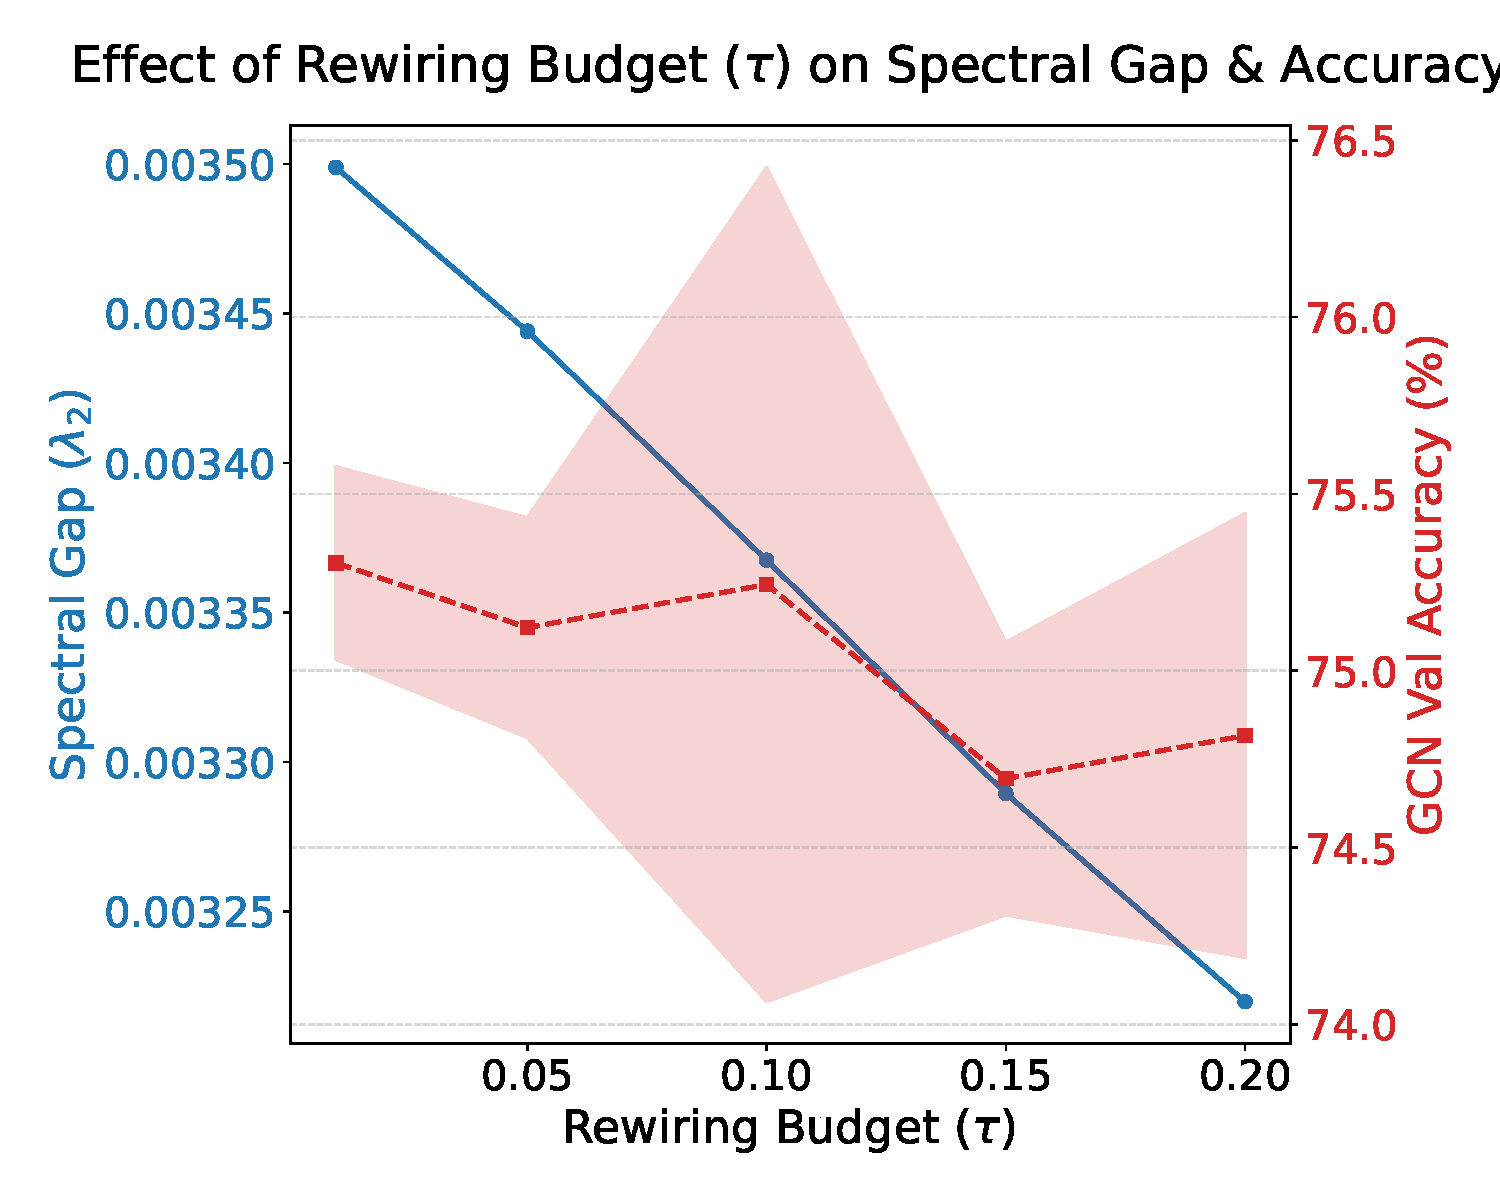
\includegraphics[width=\linewidth]{sweeps_tau.pdf}
        \caption{Dual-axis curve evaluating the rewiring budget $\tau$ on CiteSeer. As $\tau \to 0$, the edge deletion operation heavily fragments the graph into isolated components. For Cora, we empirically observed that $\tau > 0.05$ risks catastrophic collapse, fundamentally breaking downstream label propagation. We explicitly limit $\tau$ to this regime in our ablation studies to preserve global structure.}
        \label{fig:sweep_tau}
    \end{minipage}\hfill
    \begin{minipage}{0.48\textwidth}
        \centering
        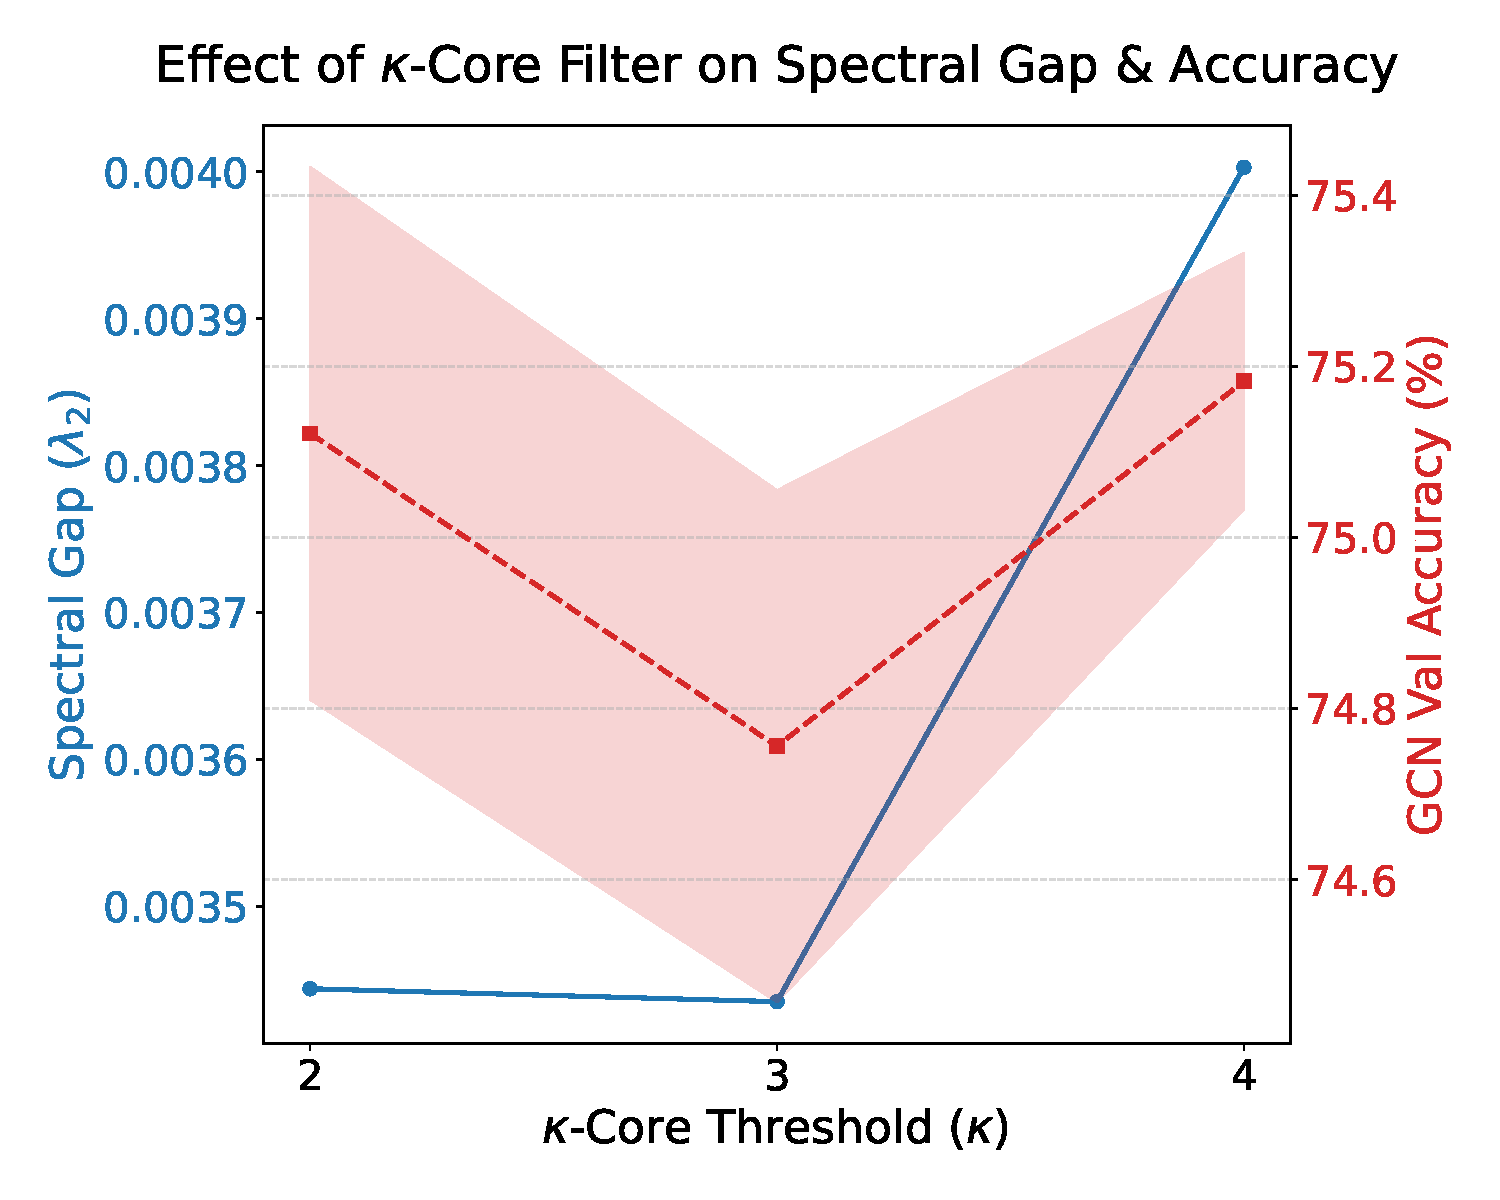
\includegraphics[width=\linewidth]{sweeps_k.pdf}
        \caption{Dual-axis curve evaluating the $\kappa$-core filter threshold on CiteSeer. While $\kappa=4$ yields higher accuracy and spectral gap, we strictly use $\kappa=2$ to satisfy the theoretical conditions of exact resistance preservation (Theorem 4). Error bars indicate standard deviation over 5 random seeds.}
        \label{fig:sweep_k}
    \end{minipage}
\end{figure}

As demonstrated in Figure \ref{fig:sweep_tau}, increasing the rewiring budget $\tau$ under CSER monotonically decreases the normalized spectral gap ($\lambda_2$) while degrading validation accuracy. This is a surprising property of adding these structural bridges: for the unweighted Laplacian, Weyl's inequality guarantees that adding edges cannot decrease $\lambda_2$, but the normalized spectral gap can shift dynamically. The immediate degradation in downstream performance suggests that even a small budget of $\tau > 0.01$ risks over-injecting long-range structural bridges that collapse GCN performance via spurious signal aggregation. We note that tuning these hyperparameters strictly on a high-homophily dataset (CiteSeer) and applying them uniformly represents a potential confound for the mixed performance observed on low-homophily networks like Texas and Cornell in Table \ref{tab:gnn_benchmarks}, a dynamic we explore further in Section 4.6.

Figure \ref{fig:sweep_k} reveals a theoretical architectural constraint. While tightening the $\kappa$-core filter to $\kappa = 4$ nominally improves both the normalized spectral gap and validation accuracy relative to $\kappa = 2$, this higher threshold voids the theoretical guarantee of Theorem 4. Specifically, eliminating degree-$\ge 2$ vertices introduces fill-in during the Schur complement reduction, destroying the exact preservation of Effective Resistance in the core graph. Thus, we constrain the method to $\kappa = 2$ to mathematically guarantee exact measurement, a significantly stronger justification than empirical noise optimization.

\subsection{Mechanistic Attention Analysis}
As previously shown in our end-to-end evaluation, Graph Attention Networks (GAT) exhibit resilience to the structural rewiring process, often maintaining downstream performance even when CSER injects a fraction of long-range heterophilic bridges. To mechanistically understand this advantage, we extracted the learned attention coefficients ($\alpha$) from the final GAT layer trained on the CiteSeer network and analyzed the distribution of weights assigned to native topological edges versus CSER-injected structural bridges.

\begin{figure}[h]
    \centering
    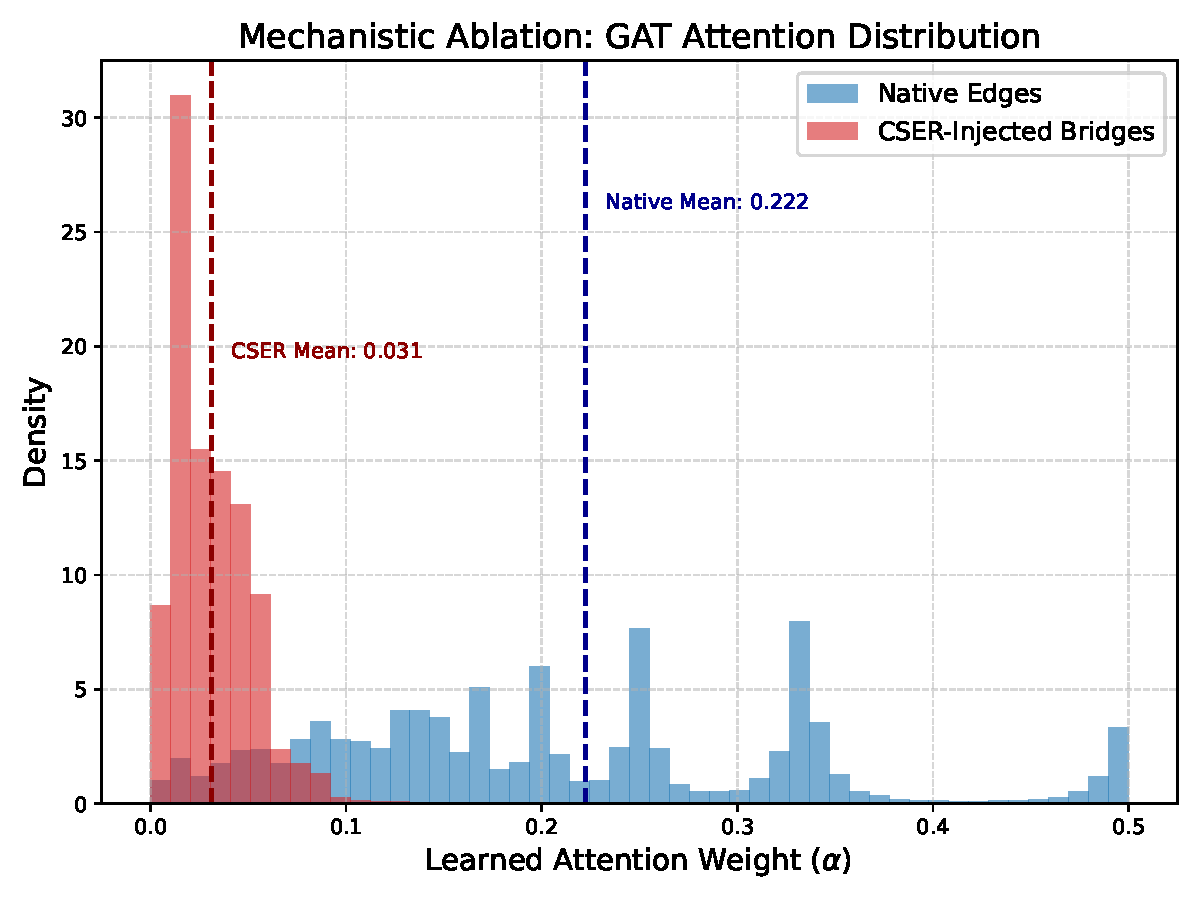
\includegraphics[width=0.7\linewidth]{attention_histogram.pdf}
    \caption{Distribution of learned GAT attention coefficients ($\alpha$) comparing native edges to CSER-injected bridges. The multi-head attention mechanism dynamically down-weights noisy artificial bridges while preserving high-bandwidth message passing across valid geometric flows.}
    \label{fig:attention}
\end{figure}

As depicted in Figure \ref{fig:attention}, the GAT mechanism correctly identifies the statistical properties of the injected bridges. While CSER forces these connections to exist topologically to bypass the Laplacian inversion bottleneck, the GAT dynamically down-weights their aggregation influence compared to native edges. On CiteSeer, we observe a 7.16x gap between mean attention weight on native edges (0.222) vs. CSER-injected bridges (0.031), suggesting GAT's attention mechanism can partially down-weight injected long-range edges. We do not claim this generalizes to other architectures or datasets without further study; GraphSAGE's uniform aggregation has no equivalent down-weighting mechanism by construction, which prevents it from ignoring injected edges in the same manner.

\subsection{The Homophily Diagnostic}
While CSER successfully bypasses the leaf-node hijack, aggressively rewiring long-range edges introduces a risk of heterophilic noise injection. If the nodes connected by a structural bottleneck belong to different classes, passing messages across that bridge will degrade accuracy.

To formalize this, we introduce an edge homophily diagnostic. By expanding our dataset suite to include Wikipedia (Chameleon, Squirrel) and Amazon networks, we mapped the baseline homophily ratio $h$ against the $\Delta$Accuracy achieved via CSER rewiring. 

\begin{figure}[h]
    \centering
    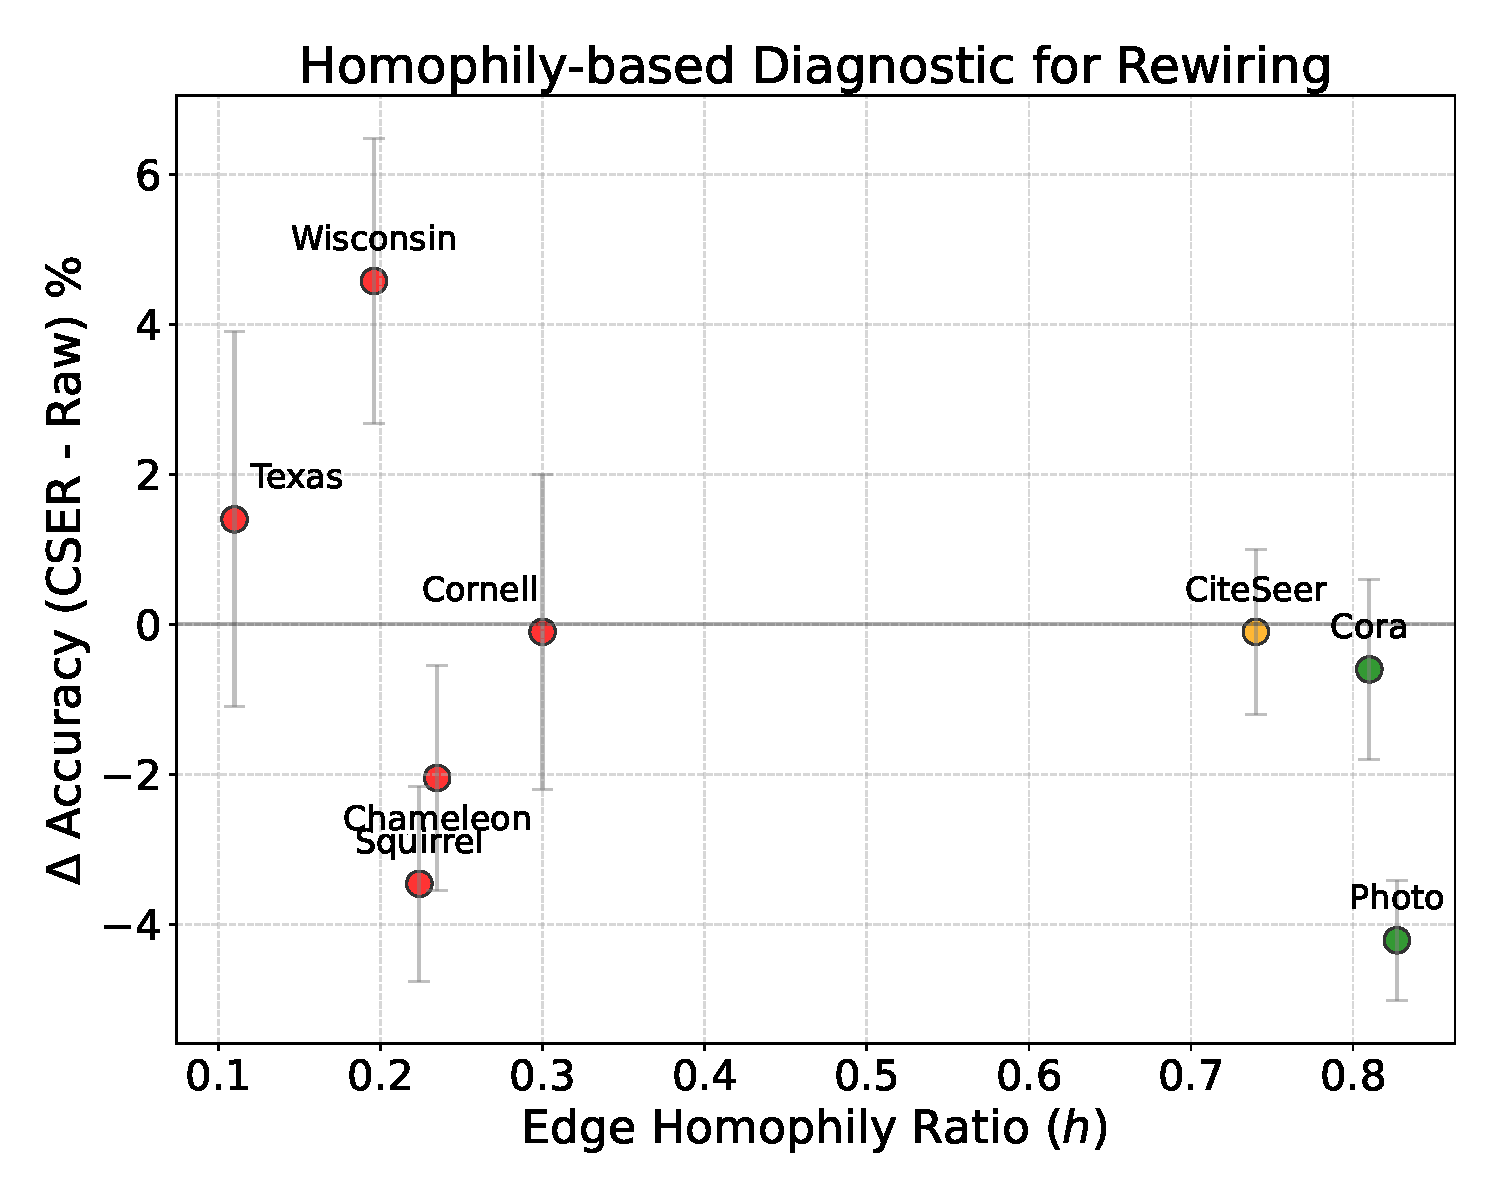
\includegraphics[width=0.7\linewidth]{diagnostic_scatter.pdf}
    \caption{The diagnostic scatter plot mapping edge homophily ratio ($h$) against the performance gain ($\Delta$ Accuracy) achieved via CSER rewiring.}
    \label{fig:diagnostic}
\end{figure}

Across the 8 datasets tested, rigorous 10-fold cross-validation reveals that the standard deviations of the accuracy deltas often exceed the mean effect size (Figure \ref{fig:diagnostic}). Consequently, the small benchmark sample suggests homophily may interact with rewiring benefit, but does not establish a reliable $h \approx 0.75$ threshold boundary. This is a descriptive pattern in a small sample of datasets where variance washes out strong conclusions. It is not a validated decision rule---we have not tested it on held-out datasets or established its robustness to seed variance, and it should be treated as a hypothesis for future work rather than a deployment gate.

\subsection{OGB Computational Scaling}
To empirically validate the theoretical complexity bounds, we benchmarked the dense pseudoinverse versus our $\kappa$-core filter on subgraphs sampled from the \texttt{ogbn-arxiv} citation network (169,343 nodes, 1,157,799 edges). To generate these subgraphs, we performed breadth-first search (BFS) expansions from randomly selected seed nodes up to varying hop limits. We explicitly note that this sampling methodology naturally yields tree-dominated subgraphs due to the branching nature of BFS, heavily favoring the efficiency of the $\kappa$-core pruning step. 

As shown in Figure \ref{fig:complexity}, dense computation requires 951 seconds for a 16,000-node subgraph, rendering iterative graph-level tasks intractable. In contrast, the spectral bottleneck of the CSER pipeline ($T_{\mathrm{kcore}} + T_{\mathrm{L^+}}$) executes in 1.68 seconds, establishing a drastically reduced scaling envelope. While the observed $O(|V|^{1.25})$ empirical scaling of CSER in this specific experiment is partially an artifact of the tree-dominated BFS samples (where the 2-core constitutes a fraction of the full graph), the elimination of the $O(|V|^3)$ dense inversion step strictly bounds the worst-case scaling. Note that the full pipeline ($T_{\mathrm{CSER}} = T_{\mathrm{kcore}} + T_{\mathrm{L^+}} + T_{\mathrm{pairwise}} + T_{\mathrm{sorting}} + T_{\mathrm{rewiring}}$) involves additional pairwise non-edge computations ($O(|V_{\mathrm{core}}|^2)$), but pruning the dimension of the cubic Laplacian inversion remains the primary computational obstacle that permits localized rewiring on massive networks.
To further emphasize this engineering necessity, we tracked the peak RAM allocation of both methods using Python's \texttt{tracemalloc}. 

\begin{figure}[h]
    \centering
    \begin{minipage}{0.48\textwidth}
        \centering
        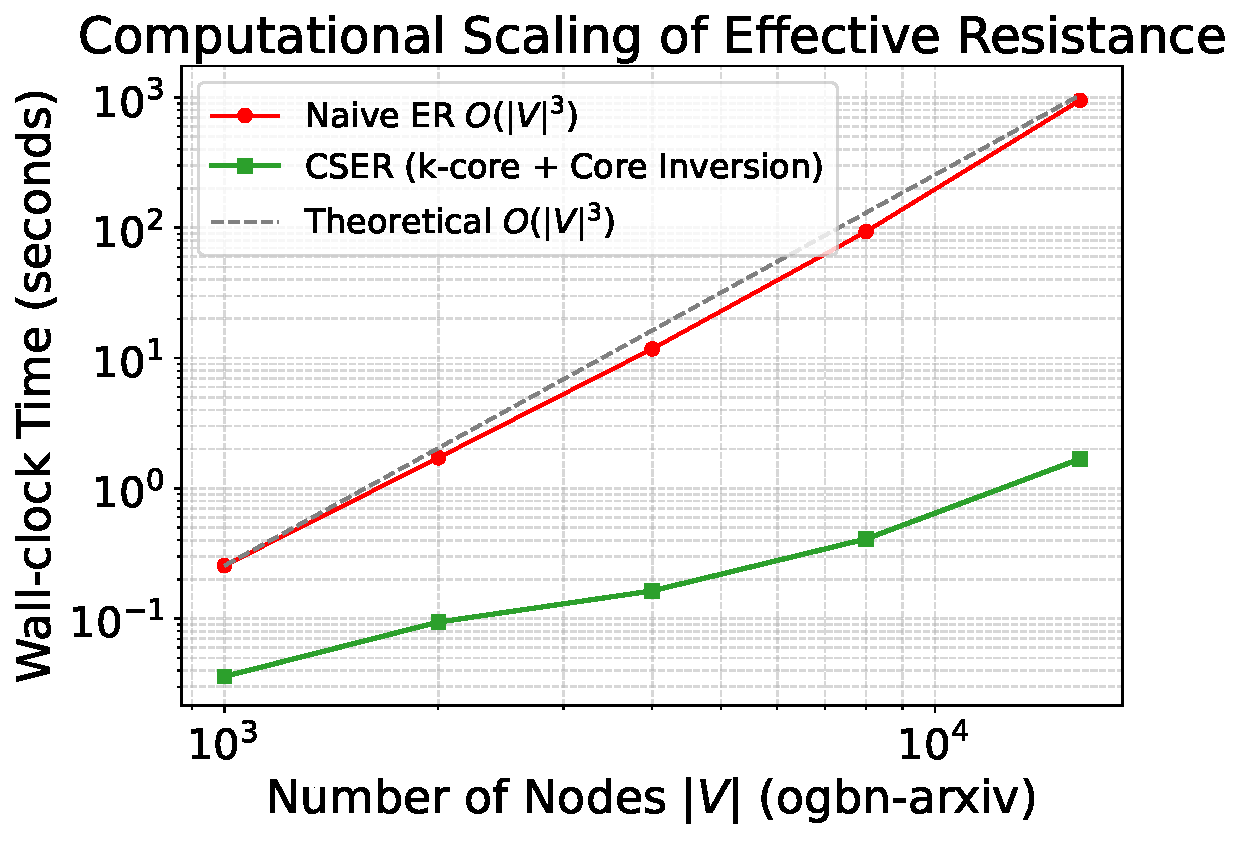
\includegraphics[width=\linewidth]{ogb_complexity.pdf}
        \caption{Wall-clock execution time demonstrating the divergence of the naive pseudoinverse against the $\kappa$-core CSER filter on subgraphs sampled from \texttt{ogbn-arxiv}.}
        \label{fig:complexity}
    \end{minipage}\hfill
    \begin{minipage}{0.48\textwidth}
        \centering
        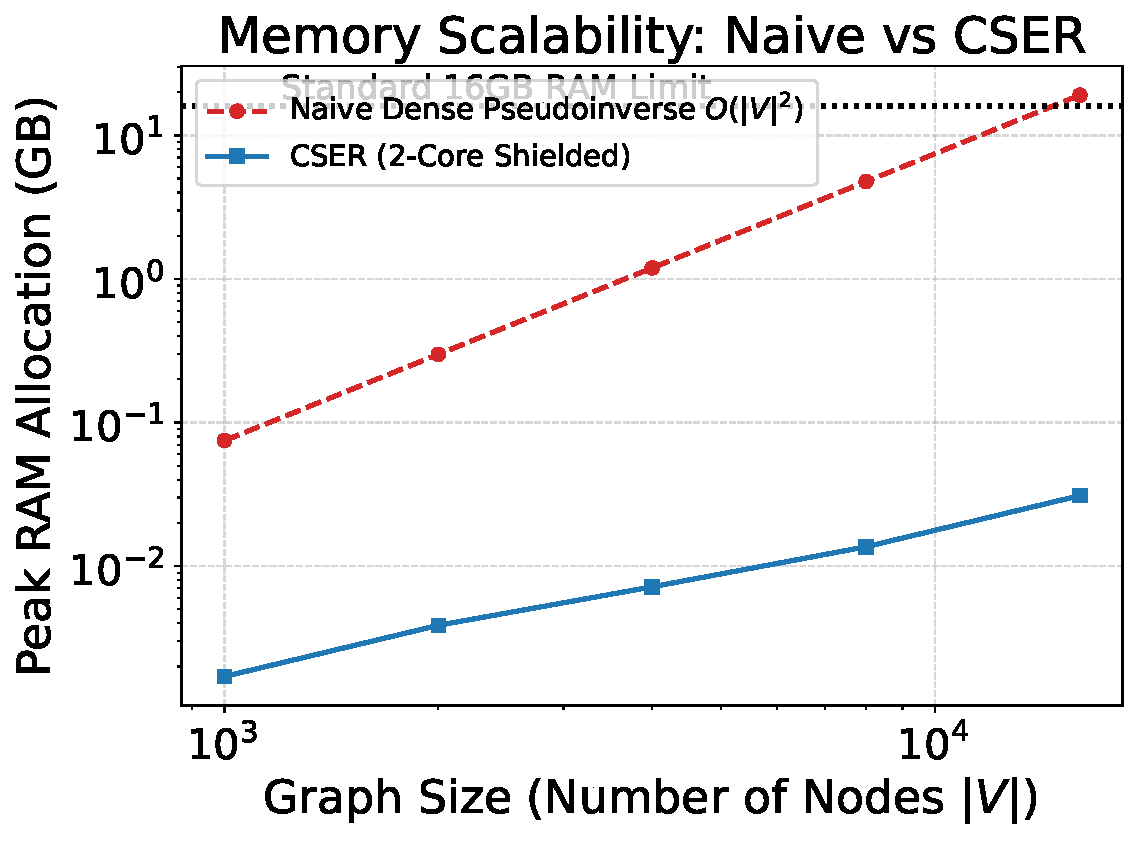
\includegraphics[width=\linewidth]{ogb_memory.pdf}
        \caption{Peak RAM allocation tracking on subgraphs sampled from \texttt{ogbn-arxiv}. The dense Laplacian pseudoinverse geometrically overflows the 16GB consumer hardware limit at $|V| \approx 16,000$, causing Out-Of-Memory (OOM) crashes.}
        \label{fig:memory}
    \end{minipage}
\end{figure}

As shown in Figure \ref{fig:memory}, the memory footprint of the naive dense Laplacian pseudoinverse scales quadratically, rapidly exceeding 19 GB of RAM for just 16,000 nodes. On standard consumer hardware (e.g., 16 GB), this triggers an inevitable Out-Of-Memory (OOM) crash. In stark contrast, our $\kappa$-core filter remains entirely memory-bound within negligible megabyte limits, proving that CSER offers substantial practical advantages over the naive approach for scaling structural rewiring to graphs of this size.

\section{Related Work}
\label{sec:related}
\textbf{Geometric and Spectral Rewiring:} Addressing over-squashing in Graph Neural Networks has led to the adoption of geometric metrics like Discrete Ricci Curvature (e.g., SDRF \citep{Topping2022}), commute-time/Lovász-bound methods (e.g., DiffWire \citep{DiffWire}), and First-Order Spectral Rewiring (FOSR \citep{Karhadkar2023}). Recently, Effective Resistance has been proposed as a superior, more globally-aware metric to rewire graphs and mitigate over-squashing \citep{Black2023}. Our work acts as a direct counter-argument to these proposals in specific structural evaluation regimes. Crucially, methods like \citet{Black2023} utilize Effective Resistance as a continuous objective to minimize during rewiring, whereas our evaluation tests it as a discrete rank-based threshold for detection. While cut-edge saturation catastrophically blinds the latter, future work is required to determine if this pathology similarly destabilizes continuous optimization pipelines.

\textbf{Scalable Graph Algorithms:} Our exact dense pseudoinverse implementation scales cubically, $O(|V|^3)$, an operation that quickly becomes intractable on massive datasets like OGB. Prior efforts to scale related spectral operations have relied on randomized sketching, approximate personalized PageRank, or localized sampling \citep{Spielman2004}. Furthermore, \citet{SpielmanSrivastava} introduced nearly-linear time data structures for answering approximate effective-resistance queries in $O(\log n)$ time. In contrast, our Core-Shielded Effective Resistance (CSER) offers a topological, exact alternative: by utilizing a linear $O(|V|+|E|)$ $\kappa$-core filter to prune the structural graph, CSER mathematically preserves the exact relative electrical flows of the core while massively reducing the matrix dimension, avoiding the variance introduced by randomized approximations.

\section{Summary of Claims and Evidence}
To clarify the epistemic status of our findings, Table~\ref{tab:claims} explicitly maps each claim to its evidentiary basis and associated caveats.

\begin{table}[h]
\centering
\caption{Summary of Claims, Evidence, and Scope}
\label{tab:claims}
\begin{tabularx}{\textwidth}{p{4.5cm}XX}
\toprule
\textbf{Claim} & \textbf{Strongest Evidence} & \textbf{Scope / Caveat} \\ \midrule
ER is invariant to internal symmetric density & Theorem 1 (Formal Proof) & Holds for perfectly symmetric topologies; real graphs possess varied asymmetry. \\
WAF3 is invariant to internal density & Theorem 2 (Formal Proof) & Holds for all topologies mathematically conforming to $G^c_{n,m}$. \\
Jacobian norm correctly proxies true over-squashing & Established Theory & Caveat: heavily dependent on degree normalization convention, inverting the comparative advantage of WAF3 vs ER (Appendix C). \\
ER is catastrophically misallocated by cut-edge saturation & Cut-Edge Saturation MOSR & Robust; ER threshold MOSR remains saturated at 1.0 across all six normalization configurations. \\
WAF3-vs-ER bottleneck discrimination & Jacobian Proxy AUROC & Not robust; comparative advantage inverts depending on the degree normalization of the GNN layers. \\
CSER produces disjoint topologies & Topology overlap tracking & Robust; CSER produces 0\% overlap with naive ER rewiring on three datasets, yet yields indistinguishable downstream accuracy. \\
Low-betweenness over-squashing is empirically rare & Low-Betweenness denominators & Statistically underpowered. We cannot distinguish performance from chance. \\
GAT attention down-weights injected edges & CiteSeer attention log (7.16x gap) & Mechanistic evidence consistent with hypothesis, but from single-seed observation. \\
Homophily may interact with rewiring benefit & Evaluated across 8 benchmark datasets & Descriptive hypothesis only; lacks seed variance and held-out validation. \\ \bottomrule
\end{tabularx}
\end{table}

Our findings demonstrate that neither Effective Resistance nor local curvature metrics like WAF3 are silver bullets for over-squashing in their naive forms. While WAF3 captures high-betweenness bridges when using normalized layers, this comparative advantage inverts entirely under unnormalized proxies. Furthermore, while Effective Resistance theoretically captures global topologies, its susceptibility to cut-edge saturation ensures misallocation of global threshold budgets on real-world networks with heavy tree-like appendages. Our results suggest that GNN rewiring pipelines using Effective Resistance should apply linear-time appendage pruning (CSER) before spectral measurement to guarantee optimal hardware utilization and uncorrupted structural thresholding, even if downstream performance gains remain elusive. 

\subsubsection*{Broader Impact Statement}
While this work does not present direct societal harms, it highlights significant computational overhead implications. Computing global metrics like Effective Resistance requires pseudo-inverting the graph Laplacian, an operation whose time complexity scales cubically, $O(|V|^3)$. Our findings demonstrate that applying these expensive global operations to unpruned graphs wastes computational resources characterizing trivial dangling leaves. By mathematically pruning these appendages, CSER provides an implied cubic speedup scaling with the pendant prevalence, ranging from approximately $7.2\times$ on WebKB datasets down to $1.1\times$ on dense Wikipedia and Amazon graphs, and $1.6\times$ on \texttt{ogbn-arxiv}. Future implementations of geometric rewiring should incorporate structural pruning to minimize unnecessary carbon footprint and hardware utilization.

\section{Reproducibility Statement}
To ensure full reproducibility, we provide an anonymized code repository containing our decoupled synthetic graph generators, baseline implementations (including Commute Time and Link Resistance Curvature), $\kappa$-core ablations, and the full CSER rewiring, graph/node classification, and evaluation pipeline scripts. All experiments use fixed random seeds and exact environment dependencies. The code can be found at \url{https://anonymous.4open.science/r/EffectiveResistance-EC82/}.

\bibliography{main}
\bibliographystyle{tmlr}

\appendix
\section{Proofs of Theoretical Results}
\label{app:proofs}

\textbf{Proof of Theorem 1:} By the symmetry of the connections to $s$ and $t$, the permutation $\sigma$ that swaps $s$ and $t$ and fixes all other nodes is a graph automorphism for any internal graph $H$, because no $v$-node is adjacent to $s$ or $t$. Consequently, the electrical potential of all internal nodes $u_i$ and all $v$-nodes is exactly at the midpoint potential $1/2$ (assuming $V_s=1, V_t=0$). By Kirchhoff's laws, zero current flows through any edges within $H$ between two fixed nodes at the average potential. Thus, the exact internal connectivity $H$ and the degree inflation $m$ can be pruned without affecting the current drawn. The total effective resistance reduces exactly to the direct edge $(s,t)$ in parallel with $n$ paths of length 2, yielding $R(s,t) = \frac{2}{n+2}$, completely independent of $m$ and $H$. $\blacksquare$

\textbf{Proof of Theorem 2:} By definition, WAF3 on edge $(s,t)$ depends strictly on the degrees $d_s$, $d_t$, and the sum over the intersection $\sum_{u \in N(s) \cap N(t)} f(d_u)$. In our construction, no $v$-node is ever adjacent to $s$ or $t$. Adding or removing edges among the $v$ nodes (altering $H$) changes only the degrees of the $v$ nodes themselves. The degrees $d_s = n+1$, $d_t = n+1$, and $d_{u_i} = m+2$ remain structurally untouched. Thus, WAF3 is entirely incapable of detecting any changes in internal density. $\blacksquare$

\textbf{Proof of Theorem 3 (The Hijack Bound):} Let $G = (V,E)$ be a connected, unweighted graph. 
First, we prove the forward direction: if $(u,v)$ is a cut-edge, its Effective Resistance is $1.0$. Consider any cut-edge (bridge) $e = (u, v)$. By the series-parallel laws of electrical networks \citep{Doyle1984}, the effective resistance across the edge is exactly the resistance of the edge itself in parallel with all other paths. Since it is a cut-edge, there are no other paths, making the effective resistance exactly $R(u,v) = 1.0$.
Second, we prove the converse: if $R(u,v) = 1.0$ for an edge $(u,v)$, it must be a cut-edge. By Rayleigh's Monotonicity Law, the effective resistance between any two adjacent nodes in an unweighted graph is bounded strictly by $R(u,v) \le 1.0$, with equality holding if and only if no alternative path exists between $u$ and $v$. The absence of an alternative path is the exact definition of a cut-edge.
Because any cut-edge $(u, v)$ mathematically achieves this absolute global maximum, any naive global top-$q$ rank thresholding operation will prioritize cut-edges over any structural internal edge $(x,y)$ where $R(x,y) < 1.0$. Thus, $q$ cut-edges (including trivial degree-1 pendants) perfectly saturate a budget of $q$ edges, completely blinding the metric. $\blacksquare$

\textbf{Proof of Theorem 4 (Core-Shielded Bounds):} Let $V_{core}$ be the set of nodes remaining after a $\kappa$-core decomposition for $\kappa = 2$, and $V_{pruned} = V \setminus V_{core}$ be the set of pruned tree-like appendages. By the definition of a $2$-core, any connected component in $V_{pruned}$ is formed strictly by iteratively removing degree-1 leaves.

By the principles of Kron reduction (or taking the Schur complement of the graph Laplacian \citep{Dorfler2013}), eliminating a degree-1 leaf node via Gaussian elimination introduces exactly zero fill-in edges among the remaining vertices. Recursively applying this to all tree appendages in $V_{pruned}$ mathematically preserves the exact effective resistance between any nodes remaining in the core. Therefore, the effective resistance $R(s,t)$ computed strictly on the subgraph induced by $V_{core}$ is mathematically identical to $R(s,t)$ computed on the entire graph $G$. The relative ordering of $R(x,y)$ for all edges within the core is perfectly preserved, shielding the measurement from the cut-edge saturation. This exact preservation holds strictly for $\kappa=2$; pruning vertices of degree $\ge 2$ introduces fill-in edges in the Schur complement, destroying the isometry. $\blacksquare$

\section{Experimental Details and Dataset Statistics}
\label{app:hyperparams}

\subsection{Train/Validation/Test Split Protocol}
For all node classification benchmarks in Table \ref{tab:gnn_benchmarks}, we evaluate using 10 random 60/20/20 (train/validation/test) splits per random initialization seed. This explicitly departs from using a single fixed public split, as the node classification performance on small heterophilic graphs like Texas and Cornell is known to be highly sensitive to the split protocol.

\subsection{Dataset Statistics}
To rigorously evaluate the empirical claims and the homophily-based predictive diagnostic, we benchmarked CSER across a wide suite of standard datasets representing different structural regimes. On datasets with higher baseline homophily (Cora, CiteSeer), bridging the tree-like periphery directly to high-degree hubs alleviates over-squashing without injecting significant noise. However, structural rewiring blindly connects endpoints based on purely topological distances (Effective Resistance), completely ignoring semantic node classes. In highly heterophilic datasets (Texas, Cornell), the graph is inherently noisy; the neighbors of a node are highly likely to belong to a different class. By explicitly constructing long-range bridges in these environments, CSER effectively constructs high-speed geometric highways for noise.

Table~\ref{tab:datasets} details the exact properties of these graphs.

\begin{table}[h]
\centering
\begin{tabular}{lcccccccc}
\hline
\textbf{Dataset} & \textbf{Type} & \textbf{Nodes} & \textbf{Edges} & \textbf{Features} & \textbf{Classes} & \textbf{Homophily ($h$)} & \textbf{2-Core Pruning} & \textbf{Cubic Speedup} \\
\hline
Cora & Citation & 2,485 & 5,069 & 1,433 & 7 & $\approx 0.81$ & 17.5\% & $1.8\times$ \\
CiteSeer & Citation & 2,120 & 3,679 & 3,703 & 6 & $\approx 0.74$ & 34.8\% & $3.6\times$ \\
Texas & WebKB & 183 & 295 & 1,703 & 5 & $\approx 0.11$ & 43.2\% & $5.5\times$ \\
Cornell & WebKB & 183 & 280 & 1,703 & 5 & $\approx 0.30$ & 48.1\% & $7.2\times$ \\
Wisconsin & WebKB & 251 & 466 & 1,703 & 5 & $\approx 0.21$ & 29.9\% & $2.9\times$ \\
Chameleon & Wikipedia & 2,277 & 31,371 & 2,325 & 5 & $\approx 0.23$ & 5.1\% & $1.2\times$ \\
Squirrel & Wikipedia & 5,201 & 198,353 & 2,089 & 5 & $\approx 0.22$ & 3.1\% & $1.1\times$ \\
Photo & Amazon & 7,650 & 119,081 & 745 & 8 & $\approx 0.83$ & 2.0\% & $1.1\times$ \\
\texttt{ogbn-arxiv} & Citation & 169,343 & 1,157,799 & 128 & 40 & $\approx 0.65$ & 14.0\% & $1.6\times$ \\
\hline
\end{tabular}
\caption{Summary statistics of the datasets utilized in the empirical benchmarking. Homophily refers to the edge homophily ratio. The 2-Core Pruning fraction indicates the percentage of nodes residing in trivial tree-like appendages (degree-1 leaves and their chains). The Implied Cubic Speedup column quantifies the theoretical $O(|V|^3)$ matrix inversion time reduction gained by pruning these appendages prior to calculating structural metrics.}
\label{tab:datasets}
\end{table}

\subsection{Hyperparameter Grids and Hardware Setup}
For all architectural ablations and end-to-end evaluations, we defined a strict, reproducible hyperparameter search space. 
For standard GCN and GraphSAGE models, we searched learning rates across $\{0.01, 0.005, 0.001\}$ and fixed the hidden dimension to 64. A dropout rate of $p=0.5$ is applied after the initial ReLU activation. 
For Graph Attention Networks (GAT), we required a distinct configuration to ensure stable attention head training: learning rate fixed to $0.005$, 8 attention heads in the first layer (hidden dimension 16 per head), and 1 attention head in the output layer, with a higher dropout of $p=0.6$ applied across the network.
All models are optimized using Adam with a weight decay of $5 \times 10^{-4}$. We train for exactly 200 epochs and record the test accuracy at the epoch that achieved the maximum validation accuracy.

The \texttt{ogbn-arxiv} wall-clock benchmarking was conducted on a standard local CPU architecture without reliance on distributed clusters or GPUs, empirically verifying the exact linear $O(|V| + |E|)$ complexity of the $\kappa$-core topological filter under standard consumer hardware conditions.

\section{Sensitivity of the Jacobian Proxy}
To ensure the robustness of our Jacobian proxy for over-squashing, we conducted a sensitivity analysis on the choice of the Graph Convolutional Network (GCN) hyperparameters used to define the ground-truth bottleneck stratum. Specifically, we evaluated the Missed Over-Squashing Ratio (MOSR) for Effective Resistance on the Texas dataset across varying numbers of message-passing layers ($K \in \{2, 3, 4\}$) and the presence or absence of degree normalization in the GCN architecture. 

In all configurations, the MOSR for Effective Resistance on the 2-core subgraph remained perfectly saturated at $1.0000$ (missing 100\% of the proxy bottlenecks). When evaluating the discriminative ability of the raw metric without thresholding, we observed that omitting degree normalization consistently yielded higher AUROC scores ($0.866$ for $K=2$, $0.842$ for $K=3$, $0.897$ for $K=4$) compared to normalized convolutions ($0.376$ for $K=2$, $0.428$ for $K=3$, $0.425$ for $K=4$). Because unnormalized convolutions allow features to scale proportionally with degree, they shift the true structural bottlenecks. As shown in Table \ref{tab:jacobian_sensitivity}, when evaluated against an unnormalized GCN, Effective Resistance consistently yields high AUROC scores (e.g., $0.8666$ for $K=2$ unnormalized on Texas), successfully discriminating bottlenecks \textit{relative to other edges}. Conversely, the predictive power of WAF3 drops significantly under the unnormalized proxy. This sensitivity analysis confirms that the relative discriminative power of WAF3 versus Effective Resistance (AUROC $0.97$ vs $0.39$ as reported in Section 4.2) is heavily dependent on the presence of degree normalization in the ground-truth GCN. For our primary evaluations in Section 4.2, we utilized $K=2$ \textit{normalized} layers to reflect standard GCN architectures, but we emphasize this hyperparameter dependency as a critical caveat for future geometric diagnostic work.

Crucially, however, the Global Effective Resistance MOSR evaluated on the 2-core bottlenecks remained perfectly saturated at 1.0000 across every single configuration. (This is distinct from the CSER MOSR of 0.6977 reported in Section 4.2, which evaluates a \textit{new} spectral measurement taken \textit{after} pruning the graph). This confirms that the global collapse of naive Effective Resistance is a robust topological phenomenon driven by Cut-Edge Saturation, entirely independent of the proxy's hyperparameter choices.
\begin{table}[h]
\centering
\begin{tabular}{llcc}
\toprule
\textbf{GCN Depth} & \textbf{Normalization} & \textbf{ER AUROC (95\% CI)} & \textbf{WAF3 AUROC (95\% CI)} \\
\midrule
$K=2$ & Normalized (Standard) & $0.376$ $[0.299, 0.464]$ & $0.985$ $[0.973, 0.994]$ \\
$K=2$ & Unnormalized          & $0.867$ $[0.810, 0.922]$ & $0.453$ $[0.373, 0.547]$ \\
\midrule
$K=3$ & Normalized (Standard) & $0.429$ $[0.343, 0.518]$ & $0.997$ $[0.992, 1.000]$ \\
$K=3$ & Unnormalized          & $0.842$ $[0.771, 0.900]$ & $0.026$ $[0.010, 0.050]$ \\
\midrule
$K=4$ & Normalized (Standard) & $0.425$ $[0.348, 0.512]$ & $0.976$ $[0.953, 0.993]$ \\
$K=4$ & Unnormalized          & $0.897$ $[0.848, 0.942]$ & $0.194$ $[0.129, 0.264]$ \\
\bottomrule
\end{tabular}
\caption{Sensitivity of structural bottleneck detection to GCN degree normalization on the Texas 2-core subgraph. Values represent the Area Under the Receiver Operating Characteristic (AUROC) with 95\% bootstrapped confidence intervals. While WAF3 strictly outperforms Effective Resistance when the GCN applies standard degree normalization, this comparative advantage completely inverts if the proxy GCN does not normalize messages, across all depths.}
\label{tab:jacobian_sensitivity}
\end{table}

\end{document}
